\documentclass{llncs}
\usepackage[utf8]{inputenc}
\usepackage{graphicx}
\usepackage{color}
\usepackage{url}
\usepackage[spanish]{babel}
\usepackage{epstopdf}

\begin{document}

%%%%%%%%%%%%%%%%%%%%%%%%%%%%%%%   TITLE   %%%%%%%%%%%%%%%%%%%%%%%%%%%%%%%

\title{Code Reimagined: Gamificación a través de la visualización de código.}

%%%%%%%%%%%%%%%%%%%%%%%%%%%%%%%   AUTHORS   %%%%%%%%%%%%%%%%%%%%%%%%%%%%%%%

\author{J.J. Asensio, A.M. Mora, \\P. García-Sánchez, J.J. Merelo}
\authorrunning{J.J. Asensio et al.}

\institute{
Departamento de Arquitectura y Tecnología de Computadores. \\
Escuela Técnica Superior de Ingenierías Informática y de Telecomunicación. \\
Universidad de Granada, España \\
\email{\{asensio, amorag, pablogarcia, jmerelo\}@ugr.es }  
}
\maketitle
%
%%%%%%%%%%%%%%%%%%%%%%%%%%%%%%%%%   ABSTRACT   %%%%%%%%%%%%%%%%%%%%%%%%%%%%%%%%%
%
\begin{abstract} 
Las herramientas de visualización de software juegan un papel muy importante en el desarrollo y mantenimiento de sistemas de software complejos. Del mismo modo, también son útiles durante el aprendizaje de los conceptos básicos de programación, los cuales son aprendidos o enseñados a edades cada vez más tempranas. En esta línea, las técnicas de gamificación que intentan hacer más atractivas las tareas de programación juegan un papel importante. Para su aplicación, es necesario establecer formas innovadoras de representación que habiliten el uso de metáforas conceptuales llamativas para el estudiante. En este trabajo se propone una herramienta de visualización de código a nivel de método, basada en mapa, utilizando videojuegos de plataformas como metáfora, en este caso, una versión libre de Super Mario Bros.
\end{abstract}


%
%%%%%%%%%%%%%%%%%%%%%%%%%%%%%%%   INTRODUCTION   %%%%%%%%%%%%%%%%%%%%%%%%%%%%%%%
%
\section{Introducción}
\label{sec:intro}
La visualización de software consiste en representar gráficamente (en 2D o 3D) de forma estática o dinámica (con animaciones) información relacionada con la estructura, tamaño, historia o comportamiento de un sistema software. El objetivo es facilitar la comprensión de diferentes aspectos del sistema. Esta visualización permite documentar complejos sistemas detectar anomalías y siendo también especialmente útil durante el aprendizaje de los conceptos. 

Para representar la estructura del software (generalmente orientado a objetos), normalmente, el enfoque consiste en representar las dependencias existentes entre las diferentes entidades. Estas dependencias puede ser modeladas como un grafo por lo que la visualización de grafos resulta adecuada. El software a un nivel más básico, es decir, a nivel de método, puede ser también representado de esta forma, mediante un diagrama de flujo. Este diagrama está basado en nodos y enlaces.

Sin embargo, el código de un método cumple además con las reglas sintácticas del lenguaje, por lo que también puede ser representado mediante su árbol sintáctico abstracto. En este árbol los nodos representan los diferentes elementos del lenguaje utilizados y las aristas su relación de inclusión (por ejemplo, el nodo IF tiene como nodos hijos la parte THEN y la parte ELSE, cada una con sus propios nodos hijos). A diferencia del diagrama de flujo, la visualización de un árbol es mucho más flexible. La jerarquía de un árbol puede ser visualizada mediante un mapa (sin utilizar flechas) \cite{softwarevisualization}.

Esta forma de visualización es susceptible de ser combinada con técnicas de gamificación \cite{kumar2012gamification}. Para ello, este trabajo propone una metáfora conceptual que consiste en utilizar el mapa de un videojuego de plataformas como representación del árbol sintáctico abstracto del programa. Esta visualización, además, permite la analogía dinámica entre ambos contextos semánticos, es decir, el protagonista del videojuego corre por el mapa y el ordenador ejecuta (corre) el programa. Esta metáfora es útil para el aprendizaje temprano de los elementos del lenguaje de programación.

Para la implementación de una herramienta de visualización dinámica de estas características se ha utilizado Java y Eclipse. El resto de este trabajo está organizado de la siguiente forma: en la sección \ref{sec:background} se explora el contexto taxonómico, se discute el concepto de legibilidad del código y su relación con algunas herramientas existentes para el aprendizaje temprano de la programación, se describen las técnicas gamificación y la importancia de su papel en la metáfora conceptual. En la sección \ref{sec:proposal} se define la herramienta propuesta concretando sus características. En la sección \ref{sec:details} se describen los detalles principales de la implementación. En la sección \ref{sec:conclusions} se establecen las conclusiones obtenidas y la continuación de este trabajo junto con los agradecimientos. 

%
%%%%%%%%%%%%%%%%%%%%%%%%%%%%%%%   BACKGROUND  %%%%%%%%%%%%%%%%%%%%%%%%%%%%%%%
%
\section{Contexto}
\label{sec:background}

%----------------------------------------------------------------------------
\subsection{Contexto taxonómico del uso de gráficos en programación}
\label{subsec:taxonomy}
Los sistemas que usan gráficos para programar, depurar y entender la computación en general han sido motivo de investigación desde el inicio de la informática. La idea de hacer más accesible la programación a cualquier tipo de usuario ha sugerido a la utilización de gráficos o lenguajes visuales para la confección de programas. De igual forma el uso de gráficos facilita la comprensión de lo que el programa hace así como su depuración cuando se enseña a programar a los estudiantes. 

En este contexto muchas veces los términos utilizados para el uso de gráficos son a menudo informales o confusos. A finales de los 80 Myers \cite{myers1990taxonomies} estableció una taxonomía más formal para los diferentes sistemas gráficos utilizados en aquel entonces y que continúa siendo válida. De esta forma establece la visualización de programas como el uso de gráficos que ilustran algún aspecto del programa o de su ejecución. En la figura \ref{fig:flowchart} se muestra un ejemplo de visualización de código de forma estática. 

En concreto se clasifican según se visualiza el código, los datos o el algoritmo. Tal visualización además puede ser estática o dinámica dependiendo de si existe algún tipo de animación mientras se ejecuta el programa \cite{urquiza2009survey}. La propuesta de este trabajo constituye una forma de visualización de código dinámica. 

\begin{figure}[ht]
\begin{center}
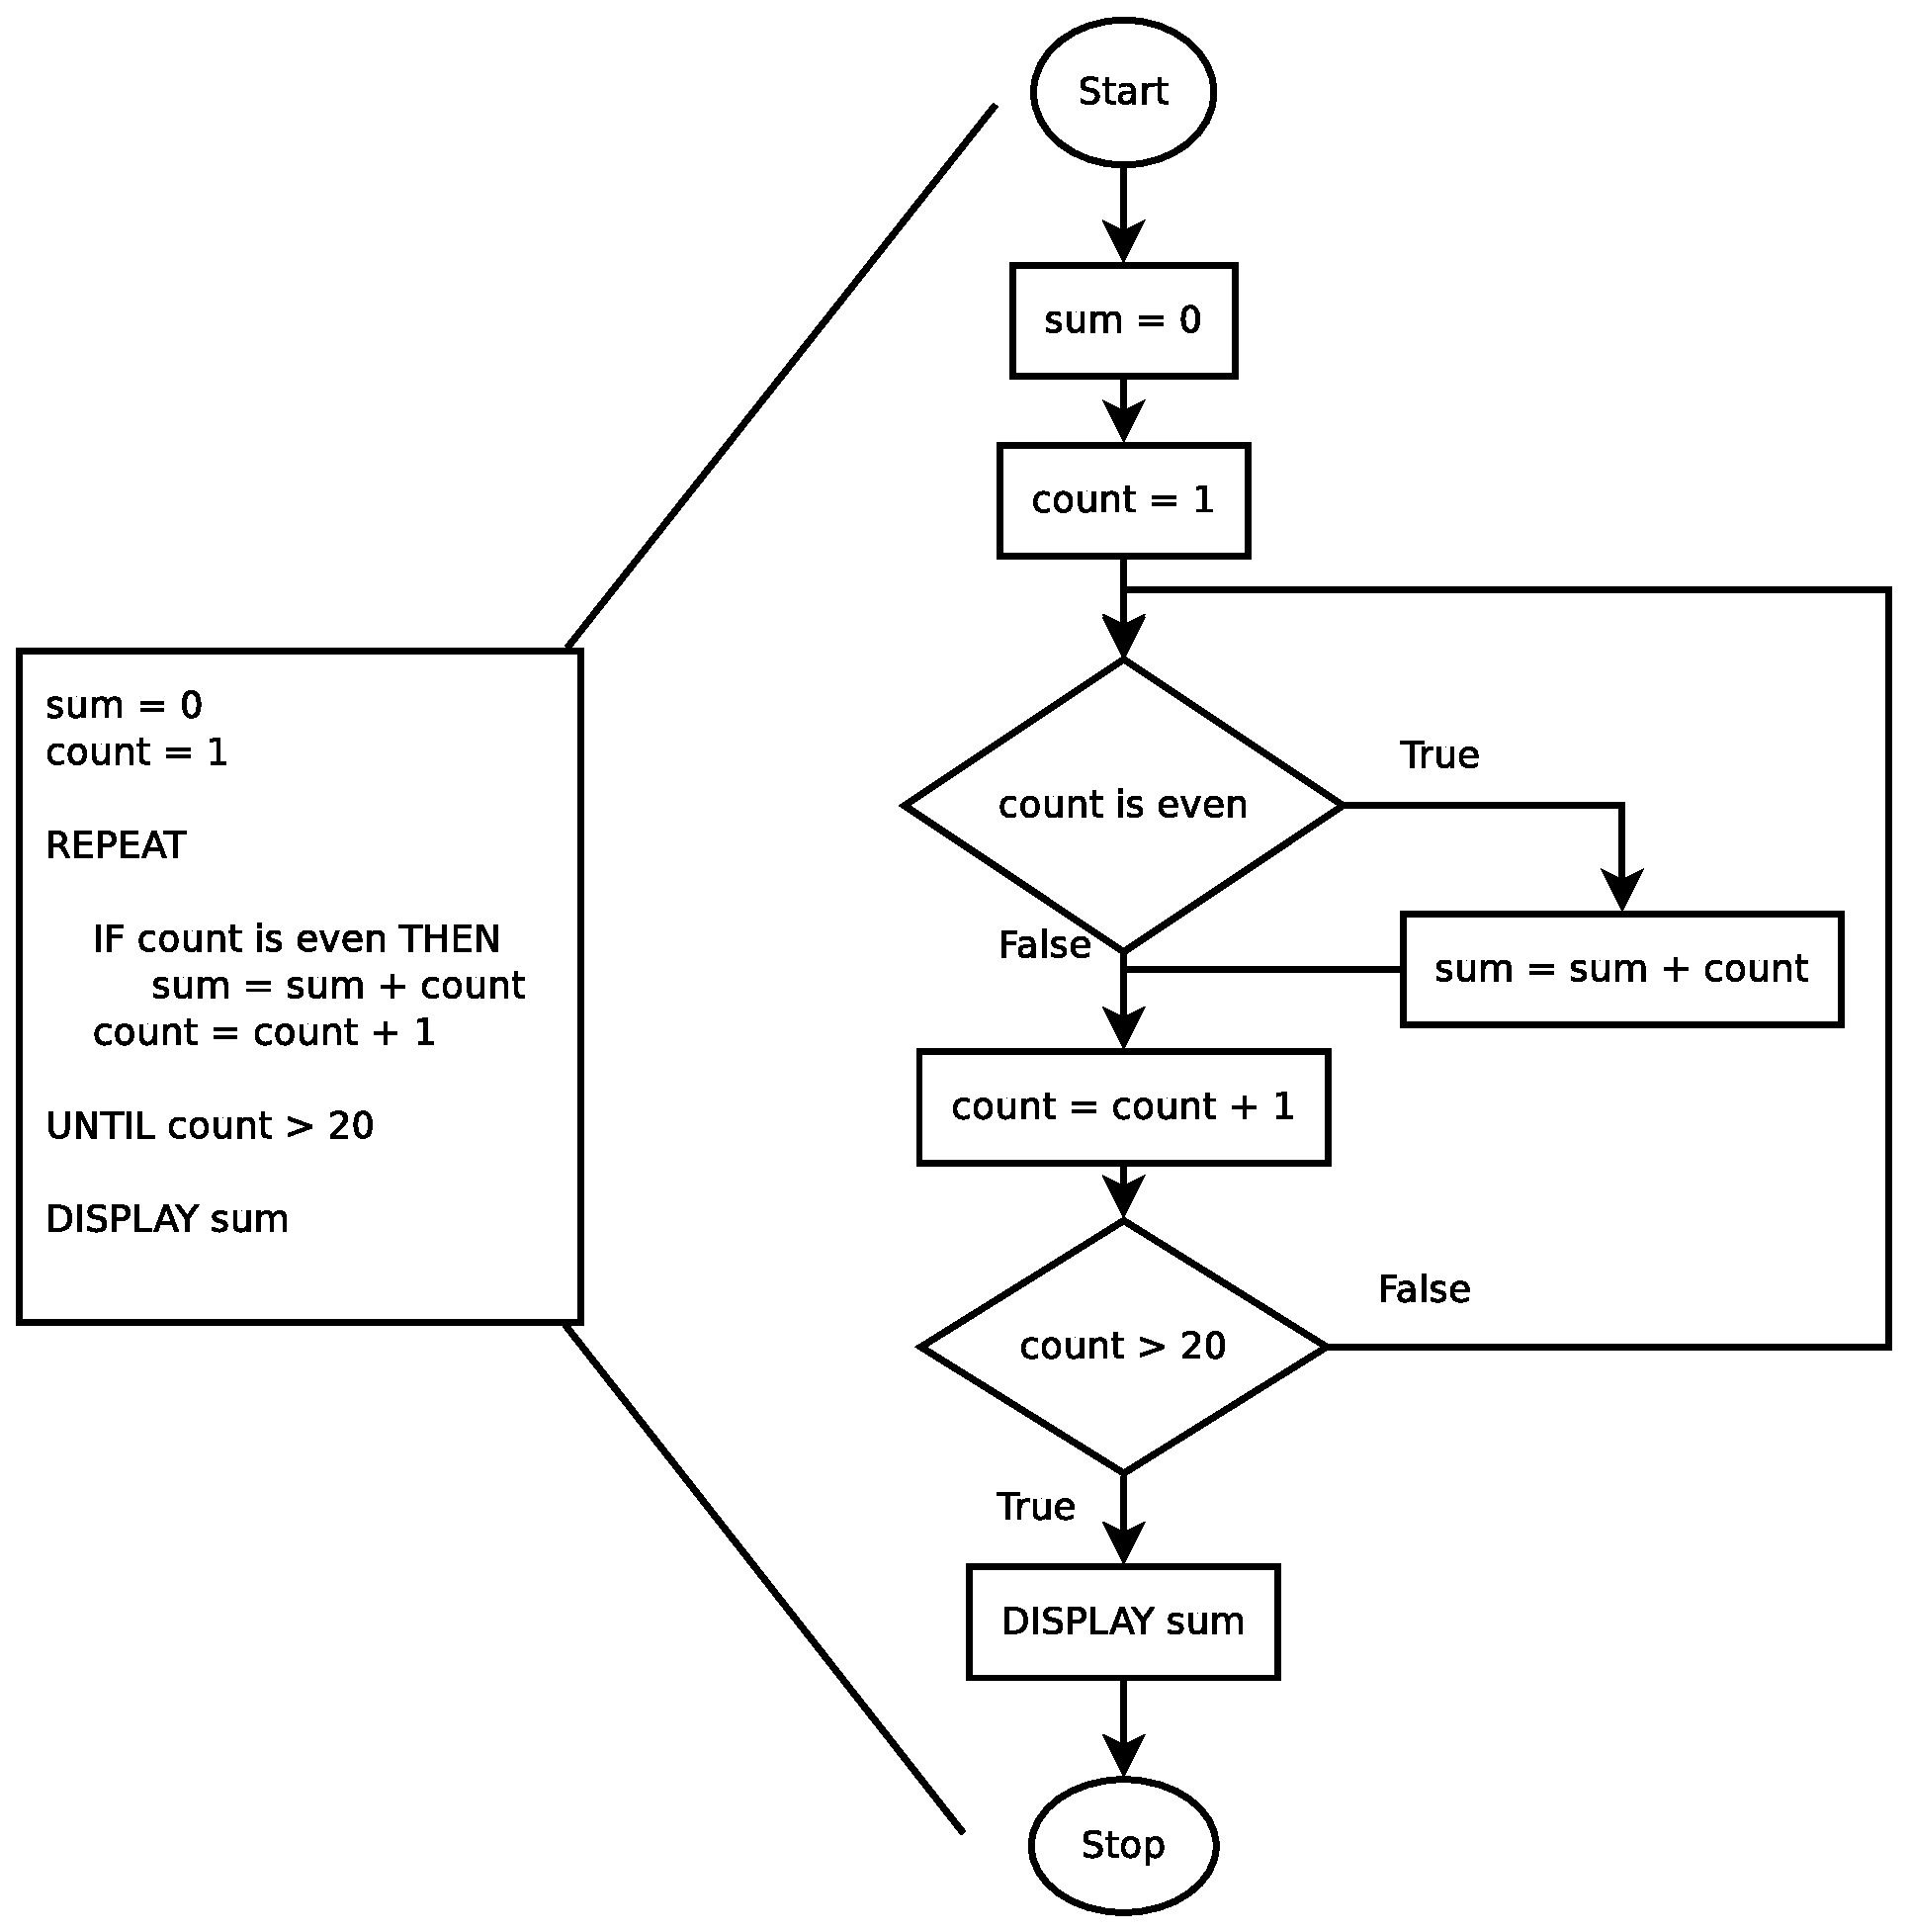
\includegraphics[scale=0.25]{images/flowchart.eps}
\caption{El diagrama de flujo visualiza el código asociado de forma estática.
\label{fig:flowchart}}
\end{center}
\end{figure}

Este trabajo, y en general la visualización de programas y la programación visual, está motivado por varias razones. El sistema visual humano está optimizado para procesar información multidimensional. La programación convencional, sin embargo, es representada como un texto unidimensional. Un atributo importante de este texto es su capacidad para que sea entendido por un humano, es decir, su legibilidad. 

%----------------------------------------------------------------------------
\subsection{Legibilidad}
\label{subsec:readability}
A menudo se hace analogía entre el texto de un programa y el texto narrativo. La legibilidad en este sentido, como concepto, es decir, la capacidad de que algo sea leído por un humano, es una idea general muy amplia. El término ``leído'' implica todas las fases del procesamiento del lenguaje a fin de que el significado sea entendido por el lector. Con esta definición en mente vemos claramente diferencias sustanciales entre la legibilidad de un texto narrativo y el código de un programa. 

La legibilidad del texto narrativo depende de la historia que se cuenta y de cómo el lector puede representar, mediante su imaginación, el significado natural de esta historia conforme a su experiencia. Si la historia es confusa o carece de sentido, el texto es poco legible. Sin embargo, es posible que la historia tenga pleno sentido y sea clara y que el texto siga siendo poco legible, por ejemplo, imaginemos un niño leyendo un artículo científico. En este caso la experiencia del lector es el factor predominante. 

Si aplicamos esta misma idea al texto de un programa, enseguida nos damos cuenta de que la ``historia'' que expresa el programa poco tiene que ver con la experiencia del lector. Su significado existe en un contexto computacional, matemático-lógico completamente distinto, generalmente abstracto, y por tanto contrapuesto, al mundo real del lector. Para que el texto del programa sea legible por tanto sólo hay dos opciones: 

\begin{itemize}
\item o bien forzamos el contexto semántico del programa para que se adecue a la experiencia natural del lector, 
\item o bien reforzamos la experiencia del lector en el contexto de la programación. 
\end{itemize}

\subsubsection{La semántica del mensaje.}
\label{subsec:message}

En el primer caso se intenta conseguir que el lector se introduzca en la programación partiendo de su experiencia natural. Su alcance, si bien importante, está limitado a la generación de programas cuya salida es multimedia y presenta alguna historia interactiva. El código usado para este fin concreto se limita a un conjunto específico de instrucciones. Incluso así, este código puede no ser legible hasta que finalmente se ejecute. 

Algunas herramientas que utilizan este enfoque son:
\begin{itemize}
\item {\em Squeak Etoys}: Es un entorno de desarrollo dirigido a niños y un lenguaje de programación basado en prototipos y orientado a objetos \cite{etoysOnline}. Dirigido e inspirado por Alan Kay para promover y mejorar el constructivismo. Los principales influyentes en esta herramienta son Seymour Papert y el lenguaje Logo. La figura \ref{fig:etoys} muestra un programa de ejemplo.


\begin{figure}[ht]
\begin{center}
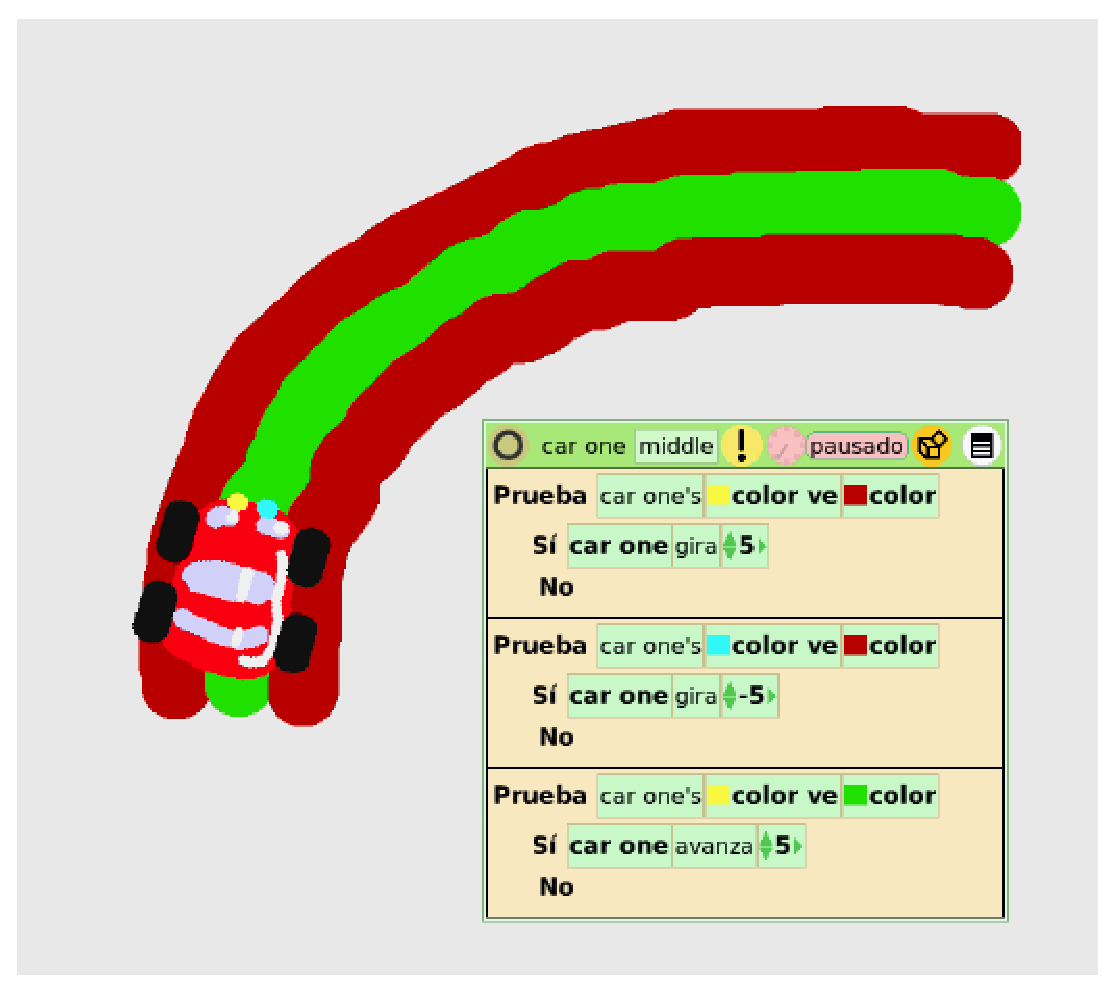
\includegraphics[scale=0.4]{images/etoys.eps}
\caption{Un programa diseñado en Etoys para controlar un coche sigue-línea.
\label{fig:etoys}}
\end{center}
\end{figure}

\item {\em Alice}: Alice \cite{AliceOnline} es un lenguaje de programación educativo libre y abierto orientado a objetos con un entorno de desarrollo integrado (IDE). Está programado en Java. Utiliza un entorno sencillo basado en arrastrar y soltar para crear animaciones mediante modelos 3D. La figura \ref{fig:alice} muestra un programa de ejemplo. Este software fue desarrollado por los investigadores de la Universidad Carnegie Mellon, entre los que destaca Randy Pausch.

\begin{figure}[ht]
\begin{center}
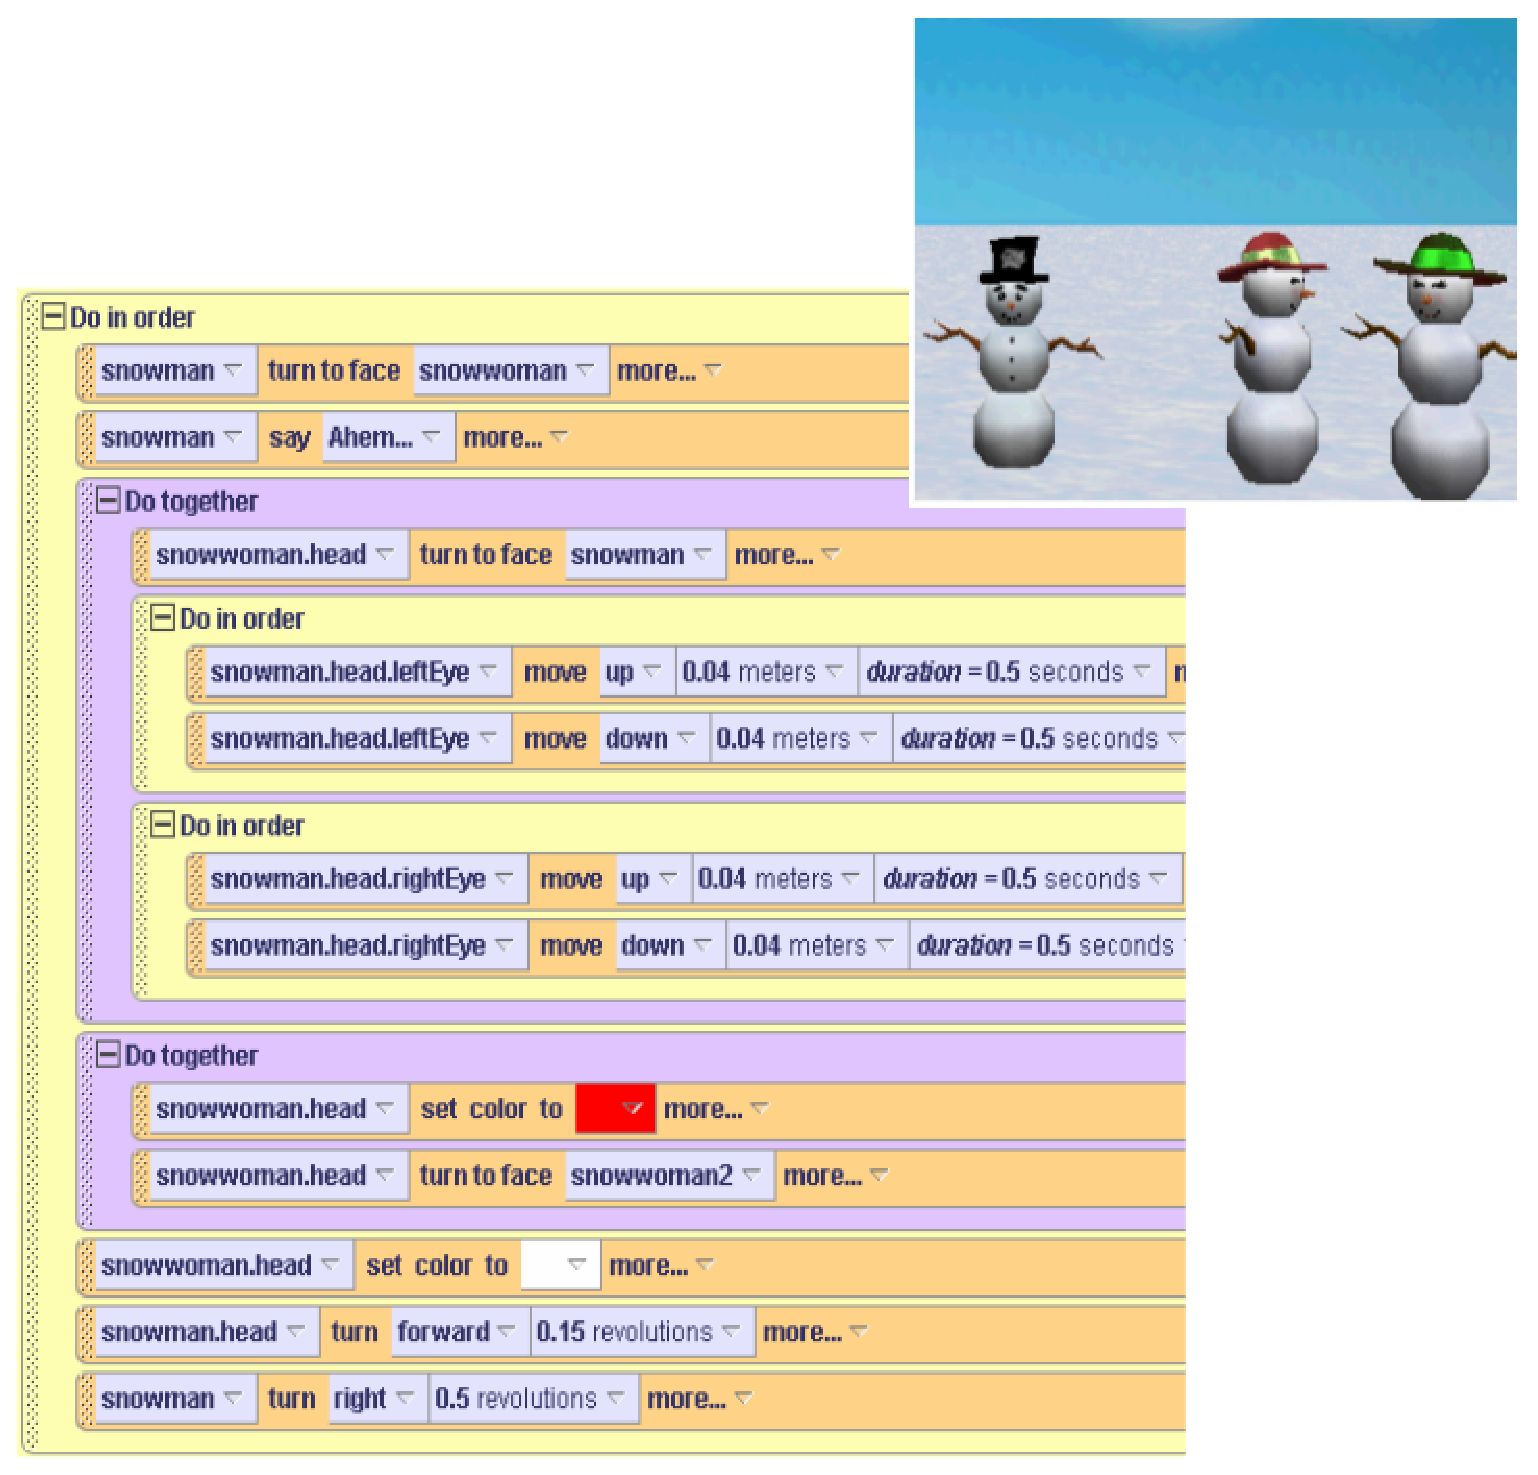
\includegraphics[scale=0.3]{images/alice.eps}
\caption{Un programa diseñado con Alice para crear una animación 3D de un muñeco de nieve. 
\label{fig:alice}}
\end{center}
\end{figure}


\item {\em Scratch}: Es un entorno de programación online \cite{ScatchOnline} que facilita el aprendizaje autónomo. Fue desarrollado por el ``the Lifelong Kindergarten group'' en el Media Lab del MIT (Massachussets Institute of Tecnology) por un equipo dirigido por Mitchel Resnick y apareció por primera vez en el verano de 2007 \cite{resnick2009scratch}. La figura \ref{fig:scratch} muestra un programa de ejemplo. Los elementos de programación son representados como bloques de distinto color que encajan entre sí.
\end{itemize}


\begin{figure}[ht]
\begin{center}
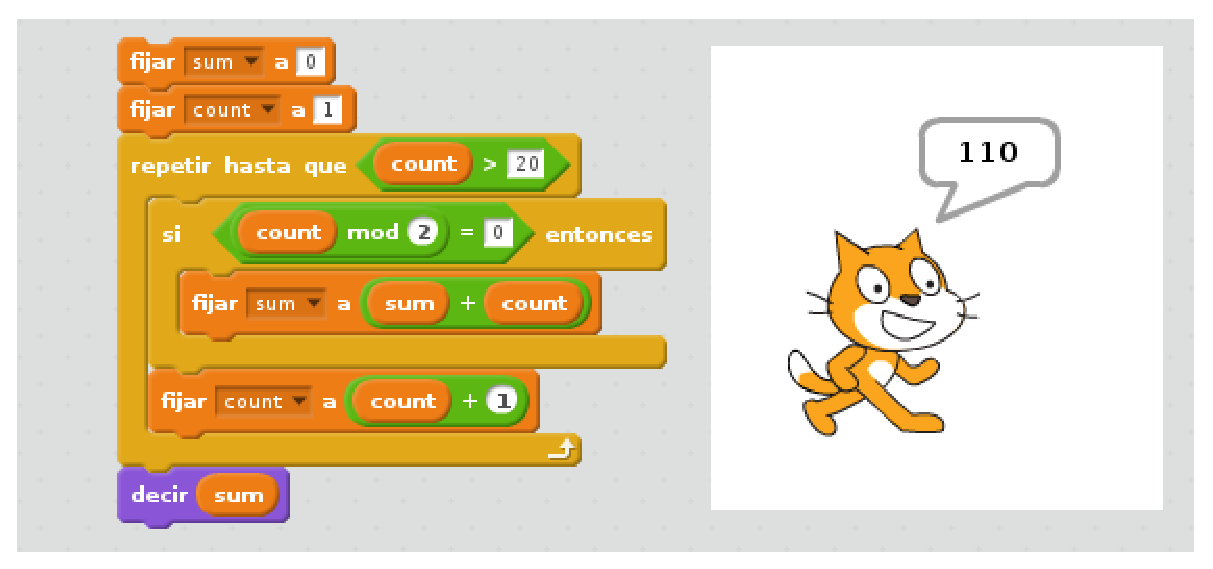
\includegraphics[scale=0.4]{images/scratch.eps}
\caption{El mismo programa de la figura \ref{fig:flowchart} diseñado con Scratch. 
\label{fig:scratch}}
\end{center}
\end{figure}


\subsubsection{La experiencia del lector.}
\label{subsec:reader}

El segundo caso, por otra parte, tiene un alcance mucho más amplio y por tanto, más difícil de conseguir. Es necesario trabajar multitud de conceptos como los algebraicos, lógicos y matemáticos desde una edad temprana en el colegio. Además, la naturaleza abstracta de estos conceptos dificulta su propia representación visual. En este sentido, algunos conceptos son más susceptibles que otros de ser visualizados, como por ejemplo, los conjuntos y sus operaciones, las funciones matemáticas, o los vectores, son más fáciles de visualizar que otros como la probabilidad, las derivadas o las diferentes partículas subatómicas. Esta visualización es importante durante el aprendizaje.

Como vemos, el concepto general de legibilidad en el ámbito de la programación no está claro. El motivo principal es claramente la confusión de no tener en cuenta que el verdadero lector de un programa no es una persona, sino una máquina. 

Desde este enfoque más amplio, es posible arrojar más luz sobre la comprensión de los procesos subyacentes en el aprendizaje de la programación. De aquí la importancia de la documentación de código \cite{tenny1988program}, a menudo descuidada. Es necesario abordar una automatización de generación de documentación legible entendiendo esta documentación, no sólo como un contenido añadido al programa, sino más bien como una característica intrínseca durante la generación del programa \cite{baecker1988enhancing}. En este paradigma el programador escribe y tanto el humano como la máquina pueden leer. Puesto que la máquina y el ser humano leen de forma diferente es necesario proveer al programador de diferentes herramientas para generar paralelamente al código, distintas representaciones semánticamente representativas. Estas herramientas son especialmente importantes durante el aprendizaje.

En este trabajo se propone una representación metafórica para visualizar el flujo de un programa de forma dinámica. La semántica utilizada para esta metáfora toma prestada la experiencia de la persona al jugar a videojuegos para hacer más intuitivo y atractivo el proceso de aprendizaje en el uso de las estructuras de control básicas de un programa escrito en un lenguaje imperativo. La representación del código en forma de juego está motivada por la aplicación de técnicas de gamificación en el contexto educativo.


%----------------------------------------------------------------------------
\subsection{Gamificación}
\label{subsec:gamification}

La gamificación consiste en el uso de mecánicas de juego o pensamiento de juego en un contexto ajeno al juego, con el fin de conseguir determinados objetivos. La gamificación aprovecha la predisposición psicológica del humano a participar en juegos. Las técnicas utilizadas consisten básicamente en tres tipos:
\begin{itemize}
\item {\em A)} Ofrecer recompensas por la realización de las tareas. 
\item {\em B)} Aprovechar la competitividad, haciendo visibles las recompensas entre los jugadores.
\item {\em C)} Hacer más atractivas tareas ya existentes que normalmente pueden ser aburridas. 
\end{itemize}

El campo de la educación presenta un gran potencial de crecimiento para la gamificación \cite{lee2011gamification}. Existen multitud de ejemplos de uso de gamificación para el aprendizaje. Quizá el más llamativo es la escuela neoyorquina Quest to Learn \cite{salen2011quest}, donde todo el proceso de aprendizaje está dirigido al juego. 

Un ejemplo concreto de gamificación aplicado al aprendizaje de programación es Code Academy \cite{codecademy}. Esta plataforma online interactiva ofrece clases gratuitas de programación con diferentes lenguajes. La técnica de gamificación usada en este contexto es la de recompensar y motivar la competitividad de los estudiantes, es decir las técnicas A) y B). 

En relación a la tercera técnica enumerada, entre muchos ejemplos, podemos destacar ParticleQuest. ParticleQuest trata de enseñar a los estudiantes de física las partículas subatómicas. La metáfora consiste en identificar las partículas subatómicas como personajes enemigos de un videojuego tipo RPG (Role-Playing Game). Las diferentes características de cada partícula identifican las habilidades y morfología de los diferentes personajes. 

\begin{figure}[ht]
\begin{center}
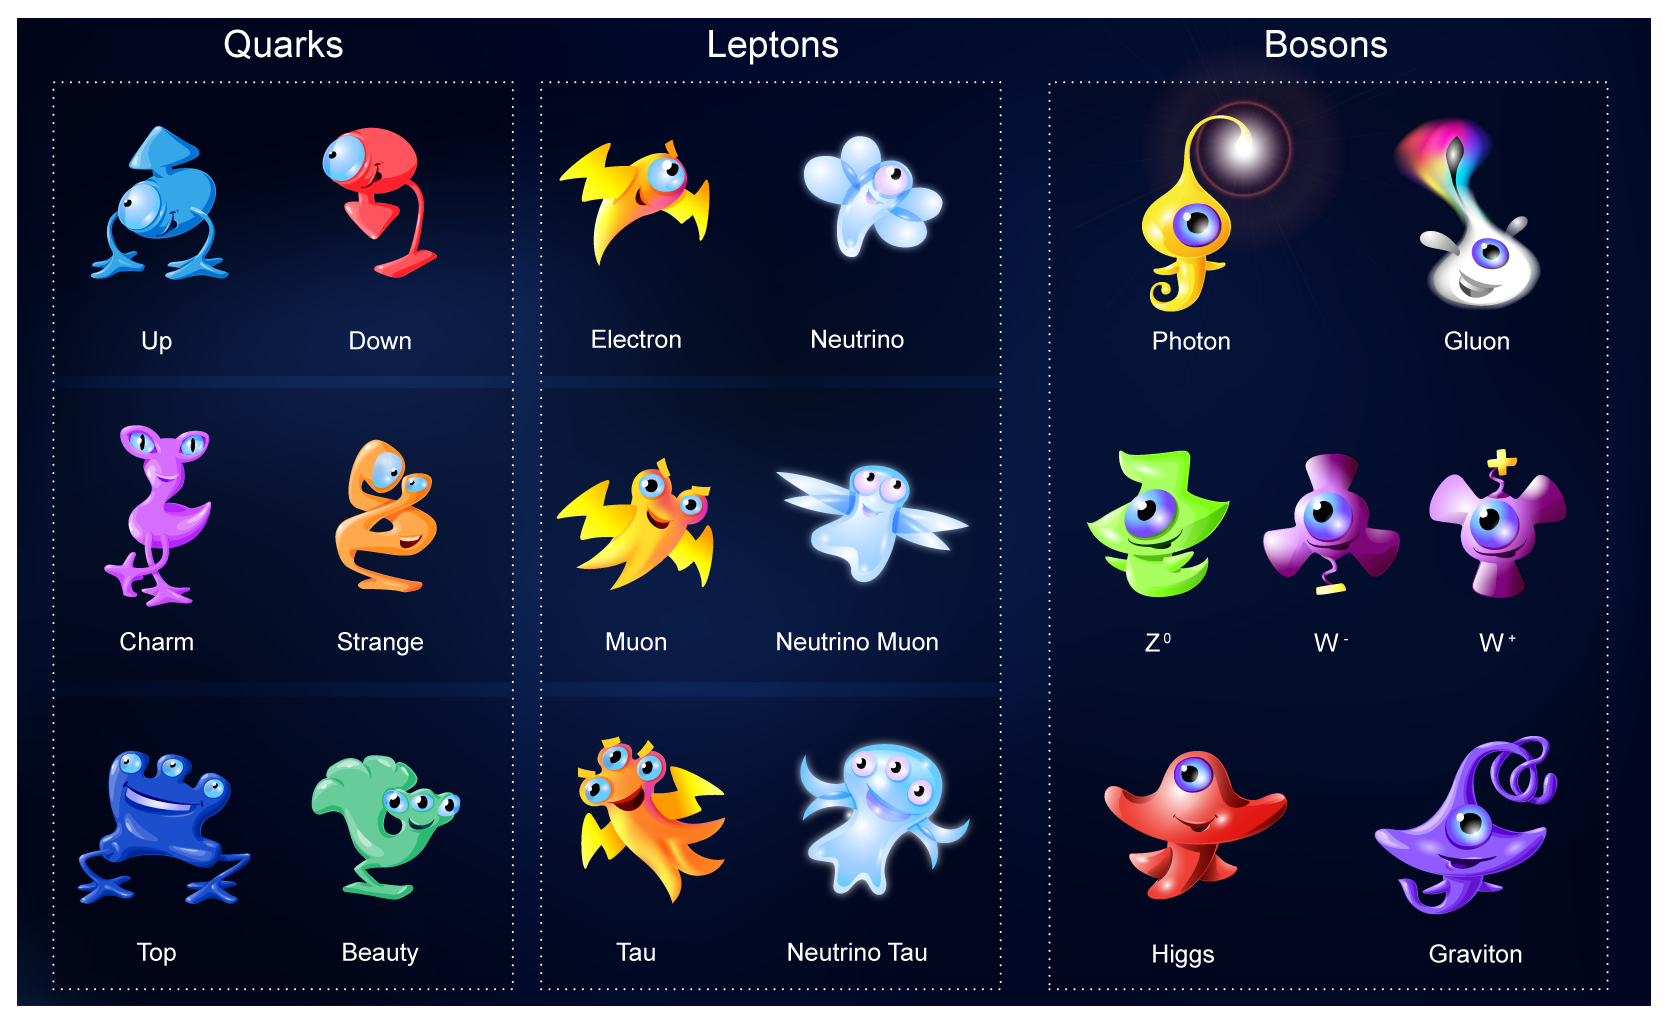
\includegraphics[scale=0.3]{images/particlequest.eps}
\caption{Ejemplo de gamificación: los enemigos en el juego ParticleQuest representan las diferentes partículas subatómicas.
\label{fig:particlequest}}
\end{center}
\end{figure}

La herramienta que se presenta en este trabajo se encuadra dentro de este tipo de técnicas. Pues al visualizar el texto correspondiente al código del programa como un escenario de un videojugo, resulta familiar y divertido al usuario, y se facilita así su comprensión e interpretación.

%----------------------------------------------------------------------------
\subsection{Metáfora conceptual}

La idea de utilizar metáforas para la representación y comprensión de conceptos abstractos es fundamental durante el aprendizaje. En matemáticas se utilizan a menudo para enseñar todo tipo de conceptos. Algunos símbolos matemáticos, como por ejemplo, los paréntesis, pueden ser interpretados como metáforas, en el sentido de que encierran explícitamente un determinado contenido. Podríamos decir que su uso como símbolo posee un significado visual añadido. Existe sin embargo un inconveniente cuando se hace un uso intensivo de estos símbolos ya que pierden su capacidad explicativa, como se observa a continuación en el siguiente programa escrito en Lisp:

\begin{verbatim}
(defun factorial (n) (if (<= n 1) 1 (* n (factorial (- n 1)))))
\end{verbatim}

Otro ejemplo es el uso de flechas para indicar transiciones de un punto a otro. Al igual que con los paréntesis, al aumentar el número de flechas, aumenta la dificultad de comprensión del diagrama. Además al ser utilizadas frecuentemente en diferentes contextos y con diferente significado, las flechas adquieren un cierto nivel de abstracción, que devalúa todavía más su capacidad aclaratoria. 

Con estos ejemplos se intenta ilustrar la importancia y necesidad de encontrar representaciones visuales más concretas que faciliten la comprensión, documentación y el aprendizaje de forma diferenciada para los conceptos que se utilizan en programación y que además puedan ser generadas automáticamente a partir del código. 

Para este propósito, es necesario conseguir un compromiso adecuado entre la abstracción asociada a los elementos visuales y su analogía semántica con el elemento representado. Además resulta también útil hacer que estas representaciones sean atractivas para el estudiante durante el aprendizaje.


%%%%%%%%%%%%%%%%%%%%%%%%%%%%%  PROPOSAL %%%%%%%%%%%%%%%%%%%%%%%%%%%%%%%%

\section{Propuesta}
\label{sec:proposal}

Este trabajo propone una representación metafórica para visualizar dinámicamente los elementos del código de un programa. La metáfora utilizada está basada en técnicas de gamificación. La idea es hacer más atractiva la tarea de codificación en programación. Para ello se utilizan videojuegos de plataformas. Quizás el videjouego de este tipo más famoso es Super Mario, para este trabajo se ha utilizado una versión libre de este juego llamada Secret Maryo Chronicles. La metáfora utilizada consiste en visualizar un método o una función, como una plataforma en el escenario del videojuego. Todo lo que hay sobre esta plataforma será el contenido del método. El uso de las estructuras de control básicas de un programa se corresponden con otras plataformas o elementos del videojuego por los que el personaje principal se mueve. Esta analogía resulta muy intuitiva puesto que relaciona la dinámica de ambos contextos. En concreto, los elementos básicos que pueden ser representados incluyen las sentencias de control típicas como el condicional, el switch, los bucles y la instrucción de retorno como se explica a continuación: 

\begin{itemize}
\item {\em Condicional}: Es representado mediante una plataforma elevada. Si la condición se cumple, el personaje saltará a la plataforma, si no, pasará por debajo.
\item {\em Switch}: Es representado mediante varias plataformas elevadas apiladas en vertical una para cada caso. El personaje saltará a la plataforma del caso que se cumpla.
\item {\em Bucle}: Es representado mediante una tubería o similar por donde el personaje se introduce y aparece al principio del bucle.
\item {\em Retorno}: Una puerta representa la devolución de datos del método.
\end{itemize}

Para que el flujo de programa pueda ser representado al menos se requieren estos elementos. Existen multitud de videojuegos de plataformas que cumplen con estos requisitos. En este aspecto la visualización puede ser personalizada por el usuario eligiendo los gráficos relacionados con el juego que le resulte más atractivo. Además, otros elementos del lenguaje pueden ser representados mediante diferentes gráficos del juego. Por ejemplo, las expresiones pueden consistir en cajas que el personaje golpea para ver su contenido. Según este esquema el programa de las figuras \ref{fig:flowchart} y \ref{fig:scratch} queda representado en la figura \ref{fig:flowchartgame}.

\begin{figure}[ht]
\begin{center}
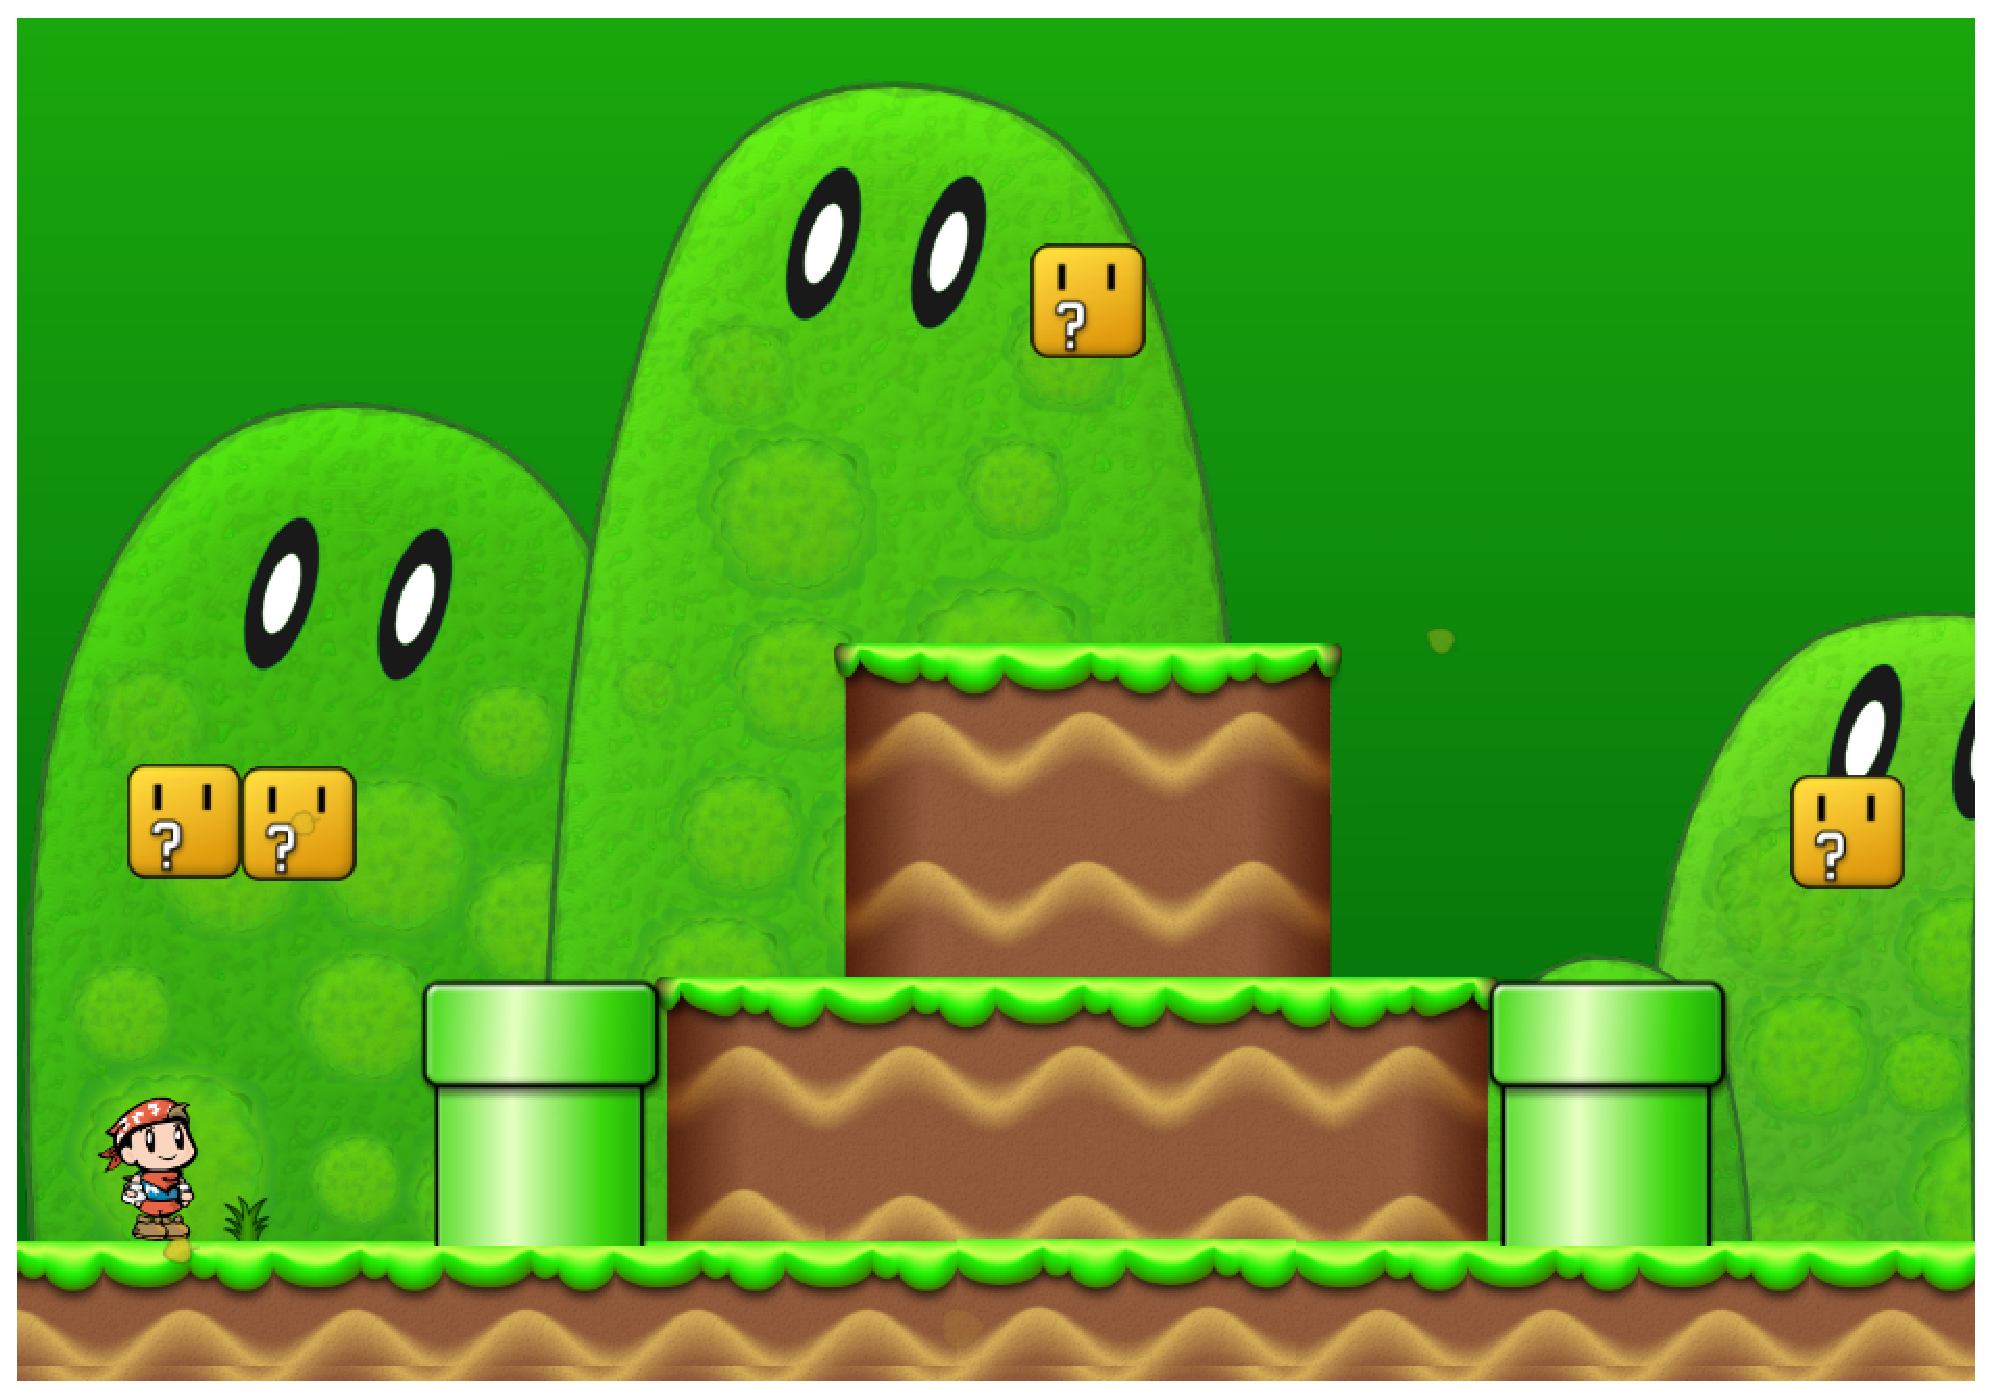
\includegraphics[scale=0.15]{images/flowchartgame.eps}
\caption{Visualización propuesta para el programa de ejemplo de la figura \ref{fig:flowchart} y \ref{fig:scratch}. El bucle está representado como la plataforma que hay entre los dos tubos, el IF dentro del bucle es otra plataforma interior y las diferentes expresiones son cajas.
\label{fig:flowchartgame}}
\end{center}
\end{figure}

Otra característica interesante para dar más capacidad de expresión a la representación visual (en el sentido opuesto al ejemplo comentado de las flechas de la sección anterior), es la posibilidad de elegir diferentes texturas para las plataformas en el contexto del juego para diferentes partes del código. Por ejemplo, supongamos que hay una parte del código más interesante o que requiere mayor atención, entonces se pueden utilizar gráficos correspondientes a escenarios más difíciles del juego como mazmorras, escenarios de lava o nieve, que sean fácilmente identificables. En la figura \ref{fig:texture} vemos un ejemplo.

\begin{figure}[ht]
\begin{center}
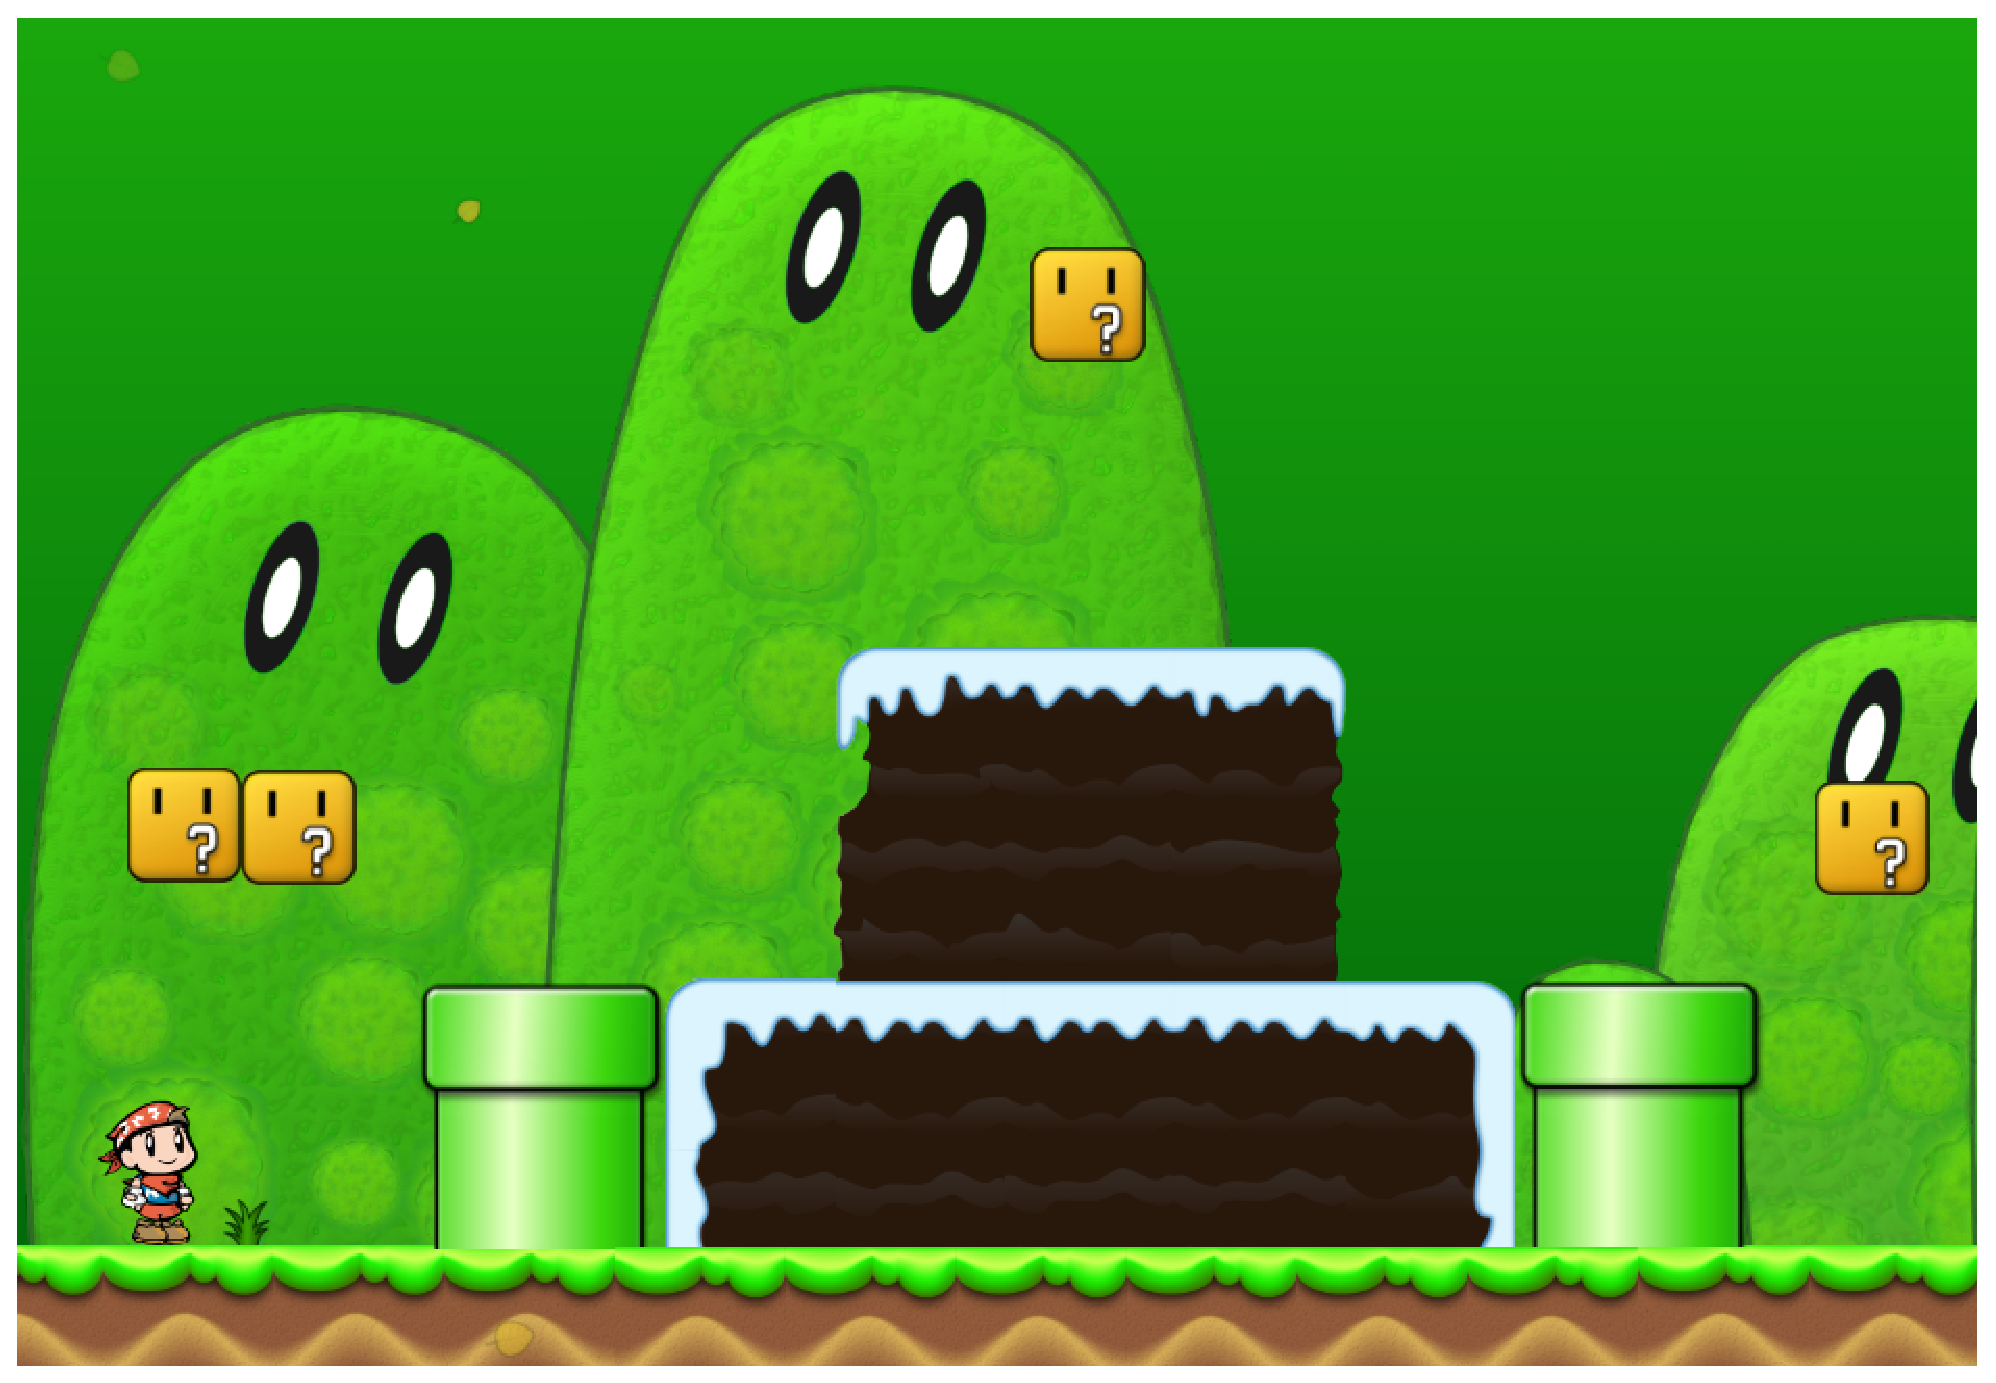
\includegraphics[scale=0.15]{images/texture.eps}
\caption{Visualización donde se ha resaltado todo el código del bucle utilizando plataformas con nieve.
\label{fig:texture}}
\end{center}
\end{figure}

El lenguaje para el que se ha implementado la herramienta de visualización propuesta es Java. El motivo de esta elección es el amplio uso del mismo, y la facilidad que poseen las herramientas de desarrollo para ser extendidas.


%%%%%%%%%%%%%%%%%%%%%%%%%%%%%  DETAILS %%%%%%%%%%%%%%%%%%%%%%%%%%%%%%%%

\section{Implementación}
\label{sec:details}
Para implementar esta herramienta de visualización dinámica se ha optado por utilizar el lenjuaje Java sobre Eclipse. Eclipse es una plataforma extensible para construir IDEs. Proporciona servicios básicos para utilizar varias herramientas que ayudan en las tareas de programación. Los desarrolladores de herramientas pueden contribuir a la plataforma envolviéndolas en forma de componentes llamados plugins. El mecanismo básico es añadir nuevos elementos de procesamiento a los plugins existentes. Mediante un manifiesto XML se describe la forma en que el entorno de ejecución de Eclipse activará y manejará las instancias del plugin. 

El plugin Code Reimagined consiste en una vista añadida a la perspectiva Java para mostrar la imagen generada a partir del código que se está editando. 

\begin{figure}[ht]
\begin{center}
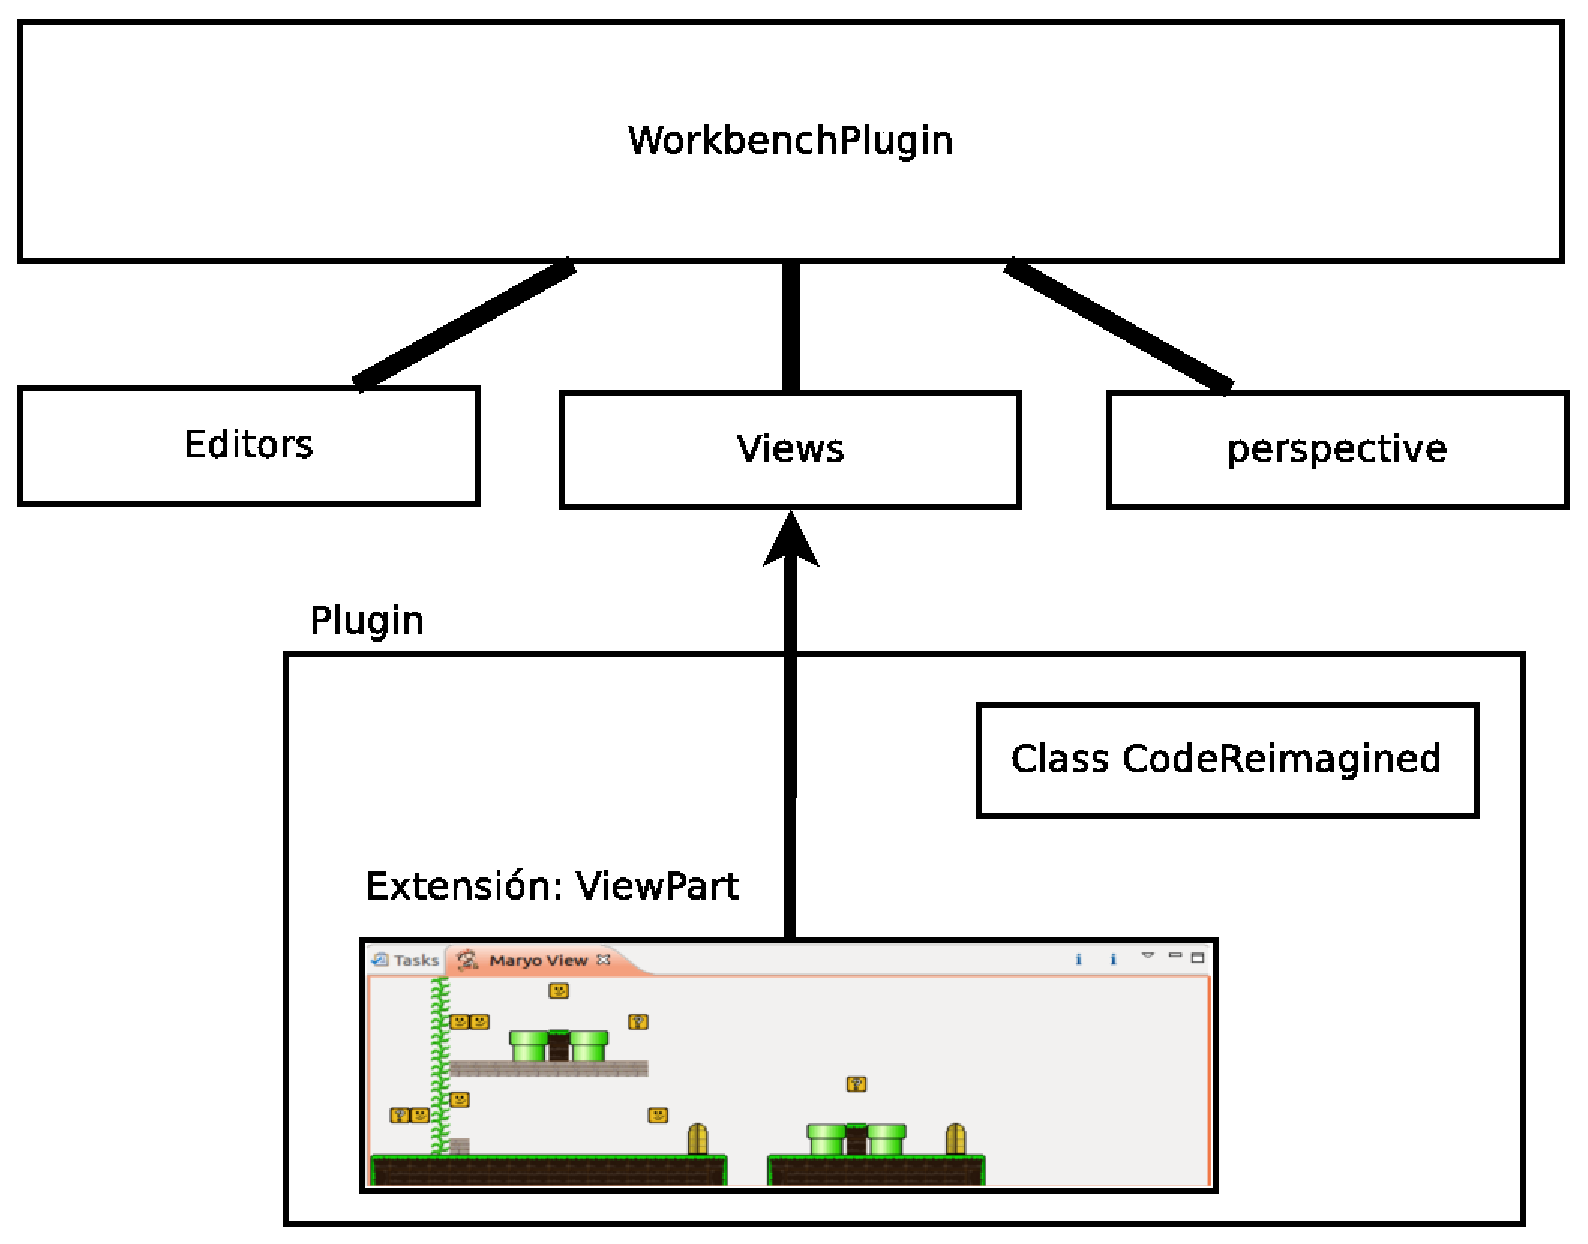
\includegraphics[scale=0.3]{images/crplugin.eps}
\caption{Esquema del plugin como una nueva vista en Eclipse.
\label{fig:crplugin}}
\end{center}
\end{figure}

Para analizar el código se ha usado el patrón ``visitor'' sobre el árbol sintáctico abstracto del código Java. Recorriendo este árbol se obtiene otro árbol cuyos nodos representan las áreas a dibujar en la vista. Estos nodos heredan de una clase abstracta y especifican cómo se pinta el elemento de programación dado y qué recuadro resulta de ello. Para obtener la imagen en la vista, basta hacer un recorrido de este árbol (sin importar el orden) y llamar al método que dibuja recursivamente los sprites de cada nodo. 

\begin{figure}[ht]
\begin{center}
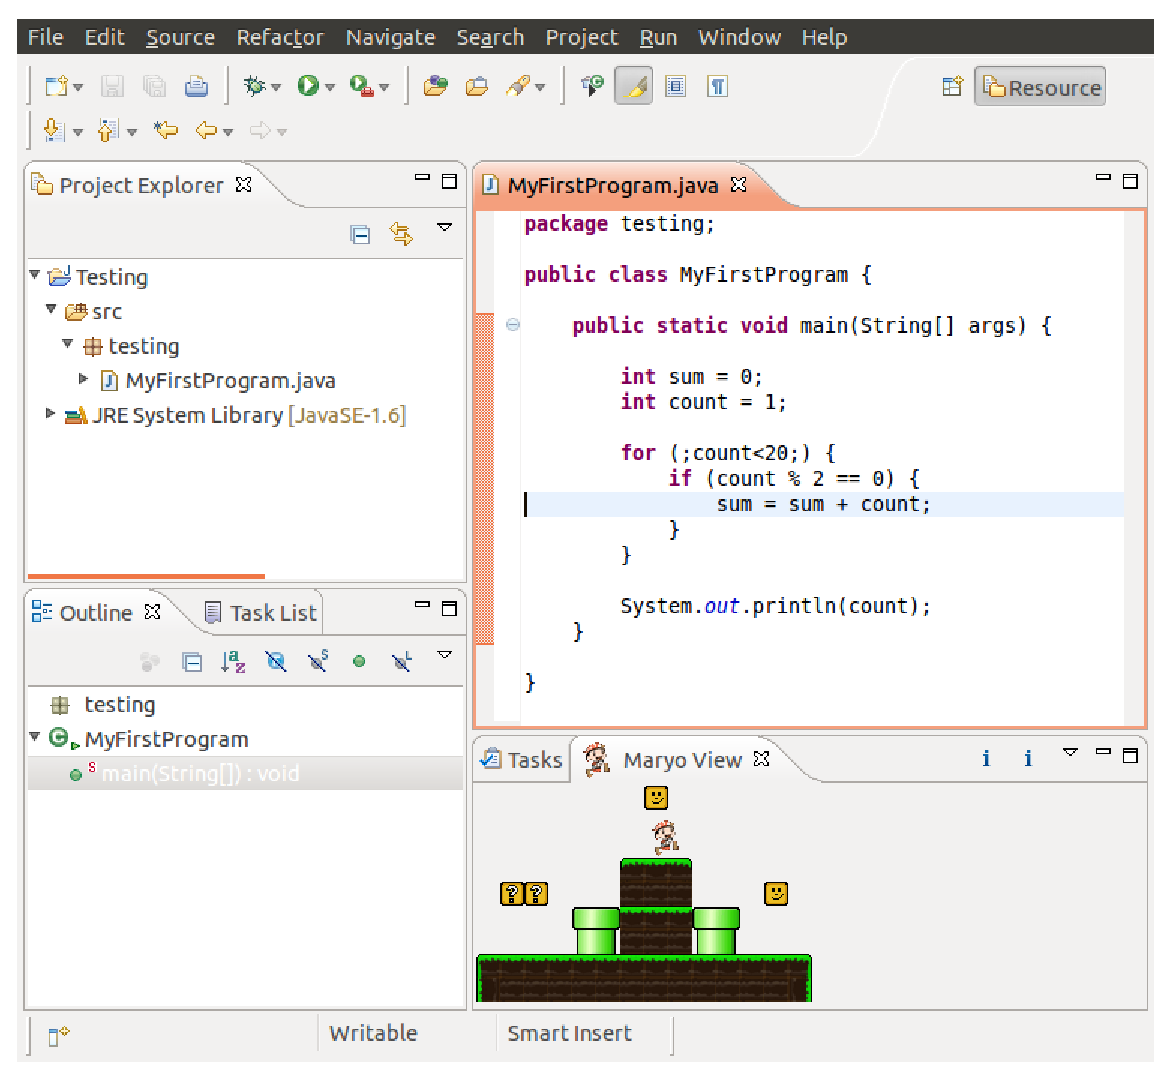
\includegraphics[scale=0.4]{images/eclipse.eps}
\caption{El plugin Code Reimagined muestra el programa de la figura \ref{fig:flowchart} y \ref{fig:scratch} una vez integrado en el entorno Eclipse. Maryo aparece sobre el área dibujada correspondiente al elemento Java que hay a continuación a partir de la posición actual del cursor.
\label{fig:eclipse}}
\end{center}
\end{figure}

Para representar la dinámica de Maryo moviéndose sobre la vista se ha implementado un ``listener'' para el cursor del editor de Java, de forma que el personaje aparecerá en el área correspondiente al elemento Java que haya inmediatemente después (figura \ref{fig:eclipse}). La manera de hacerlo ha sido utilizar una tabla hash indexando los nodos correspondientes a los elementos Java según su offset en el archivo.

Otra funcionalidad implementada es el posicionamiento del cursor en el editor Java, al hacer doble clic sobre el elemento correspondiente del mapa.

Este plugin se presentó al VII Concurso Universitario de Software Libre \footnote{\url{www.concursosoftwarelibre.org}} quedando finalista en la final local de la Universidad de Granada. El código está disponible para descarga en \url{https://github.com/javiplay/code-reimagined}.


%%%%%%%%%%%%%%%%%%%%%%%%%%%%%  CONCLUSIONS %%%%%%%%%%%%%%%%%%%%%%%%%%%%%%%%

\section{Conclusiones}
\label{sec:conclusions}

En el contexto taxonómico de la visualización de programas y partiendo del concepto de legibilidad del código, este trabajo ha identificado la necesidad de desarrollar técnicas de visualización automáticas, donde la metáfora conceptual juegue un papel básico, no sólo para el aprendizaje sino también para la documentación y la comprensión de las tareas y conceptos relacionados con la programación. 

Para este tipo de visualización se ha establecido un principio básico de diseño que consiste en maximizar la precisión semántica de las representaciones minimizando la pérdida de analogía con los conceptos representados.
Para la aplicación de este principio se ha comprobado la utilidad de las técnicas de gamificación, concretamente el uso de videojuegos de plataformas para representar el flujo de un programa.

La representación propuesta es independiente del lenguaje y por tanto, complementaria a cualquier software de programación y especialmente adecuado para herramientas de aprendizaje constructivista como Scratch. Una vez concretados los detalles de esta representación, se ha desarrollado una herramienta de visualización dinámica de código Java en forma de plugin para Eclipse. 

Como líneas de actuación futura, además de añadir nuevas características, se propone la realización de experimentos para validar la efectividad de esta herramienta. En caso de obtener resultados positivos, se podría aplicar esta forma de visualización ``gamificada'', a otro tipo de diagramas relacionados con la programación orientada a objetos. 



%%%%%%%%%%%%%%%%%%%%%%%%%%%%%  ACKNOWLEDGEMENTS %%%%%%%%%%%%%%%%%%%%%%%%%%%%%%%%

\section*{Agradecimientos}
Este trabajo ha sido apoyado por el proyecto de excelencia EVORQ con referencia P08-TIC-03903 de la Junta de Andalucía, el proyecto Anyself con referencia TIN2011-28627-C04-02 del Ministerio de Innovación y Ciencia y el proyecto 83, CANUBE, concedido por el CEI-BioTIC de la Universidad de Granada.

\bibliographystyle{splncs}


\bibliography{bibliography}


\end{document}


